% ANEXO------------------------------------------------------------------------

\begin{anexosenv}
\partanexos

% Primeiro anexo---------------------------------------------------------------
\chapter{Nome do anexo}     % edite para alterar o título deste anexo
\label{chap:anexoA}

Lembre-se que a diferença entre apêndice e anexo diz respeito à autoria do texto e/ou material ali colocado.

Caso o material ou texto suplementar ou complementar seja de sua autoria, então ele deverá ser colocado como um apêndice. Porém, caso a autoria seja de terceiros, então o material ou texto deverá ser colocado como anexo.

Caso seja conveniente, podem ser criados outros anexos para o seu trabalho acadêmico. Basta recortar e colar este trecho neste mesmo documento. Lembre-se de alterar o "label"{} do anexo.

Organize seus anexos de modo a que, em cada um deles, haja um único tipo de conteúdo. Isso facilita a leitura e compreensão para o leitor do trabalho. É para ele que você escreve.

% Novo anexo-------------------------------------------------------------------
\chapter{Coleta de Amostra do Solo}
\label{chap:anexoColeta}

É o processo de obter amostra de terra, de tal forma que esta seja a que mais represente o terreno onde será implantada uma cultura. Esse procedimento é realizado devido ao fato de que toda a recomendação de adubação é calculada considerando que a amostra represente fielmente todo o talhão.

\begin{figure}[H]
    \centering
    \caption{Coleta de Amostra do Solo}
    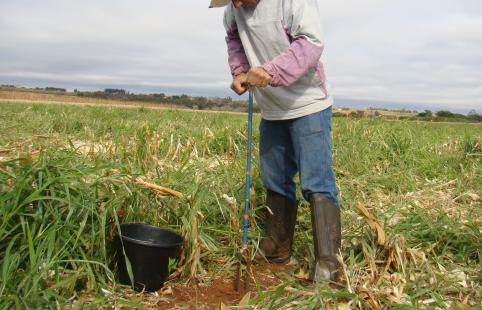
\includegraphics[width=13cm]{./dados/figuras/coleta_de_amostra_do_solo.jpg}
    \label{fig:coletadeamostra}
    \fonte{Sílvia Zoche Borges}
\end{figure}


\chapter{Laudo Técnico do Solo}
\label{chap:laudodosolo}

O laudo técnico do solo é um documento emitido por um laboratório especializado. Nele estão contidas informações sobre os nutrientes da terra e seus teores.

\begin{figure}[H]
    \centering
    \caption{Laudo Técnico do Solo}
    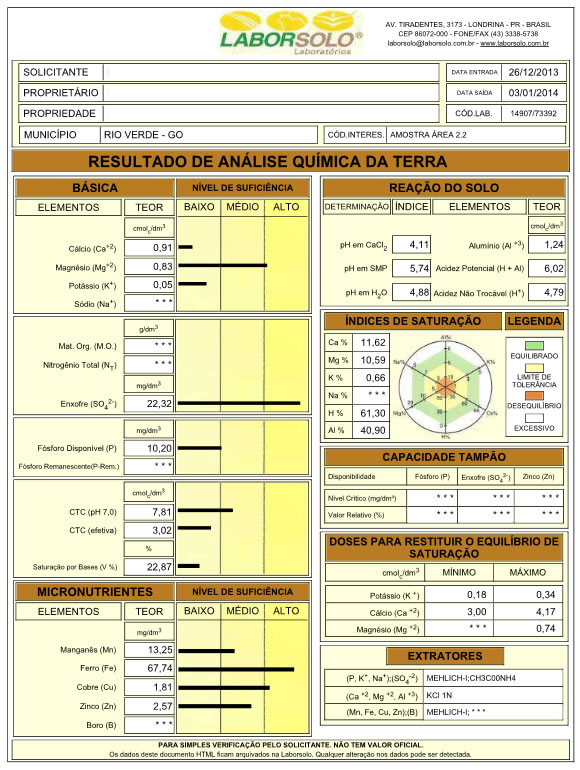
\includegraphics[width=13cm]{./dados/figuras/ex_analise_quimica.jpg}
    \label{fig:laudotecnico}
    \fonte{Roberto Antunes Fioretto}
\end{figure}


\end{anexosenv}
